% quantgravbits.tex - the concise quantum-gravity paper, trimmed from quantgravalt.tex.
% Build:  make bits   (writes build/quantgravbits.pdf; needs latexmk and pdflatex; no numbers file needed).
% Numbers are written in the text.  Those of Sections 3 to 6 come from the scripts of the qwla repository named in each
% result (generic_phase.py, exact_window.py, hat_flips.py, ring_bits.py, qdeform_punctures.py, hat_chirality.py,
% spectre_fold_flips.py); those of Section 2 and Result 9 are from quantgravalt.tex and the code of this repository.
\documentclass[11pt]{article}
\usepackage[T1]{fontenc}
\usepackage[utf8]{inputenc}
\usepackage{amsmath,amssymb,amsthm}
\usepackage{mathtools}
\usepackage[a4paper,margin=26mm]{geometry}
\usepackage{graphicx}
\usepackage{xcolor}
\usepackage{enumitem}
\usepackage{url}
\usepackage[hidelinks]{hyperref}
\usepackage{orcidlink}
\graphicspath{{figures/}}

\newcommand{\exact}{\textbf{\textsc{Exact}}}
\newcommand{\numeric}{\textbf{\textsc{Numeric}}}
\newcommand{\negres}{\textbf{\textsc{Negative}}}
\newcommand{\defn}{\textbf{\textsc{Definition}}}
\setlength{\emergencystretch}{3em}
\theoremstyle{definition}
\newtheorem{result}{Result}

\title{Geometry Bits on Aperiodic Monotiles:\\ Open Flips in the Plane, Closed Flips on the Sphere, and Their Quantisation}
\author{Brent Hartshorn \orcidlink{0009-0004-2853-655X}, Tristan Romanov and James Lockwood}
\date{\today}

\begin{document}
\maketitle

\begin{abstract}
\noindent We build a discrete model of quantum geometry from tilings by the hat and Spectre monotiles and ask what it has that a quantum-gravity model needs. In the plane a phason flip of the Spectre tiling, computed with an exact test of the fractal window, is never a local move: it is a ribbon of tiles that crosses every region tested, out to radius $100$, conserves the number of bump-and-dent pair qubits per unit length, and changes them only where its tiles sit on the lower edge of the window. On a closed surface the picture inverts. The Goldberg sphere $GP(3,0)$ has exactly $2^{12}$ hat tilings, one bit per cone point, every flip is a closed ring of five tiles around a cone point, and the vertex count is an exact nearest-neighbour function of the bits. Read as spins, the bits contain the gauge-invariant space of a sphere with twelve spin-$\tfrac12$ punctures, and the vertex count becomes the Heisenberg model on the icosahedron there. That model is the classical limit of a family obtained by the skein quantisation used for wild embeddings; at level $2$ it is a free Majorana model with the same flux through every face. The hat's handedness is visible in the bits through a four-bit term on helical paths, but it cannot fix the sign of that flux: the tiling breaks mirror symmetry, and the flux also needs time reversal broken.
\end{abstract}

%------------------------------------------------------------------------------------------------------------------------------------
\section{Introduction}\label{sec:intro}
Discrete approaches to quantum gravity need a substrate whose elementary changes are local and reversible, a space of states on which those changes act, and a Hamiltonian that ties the states to geometry. Aperiodic tilings come with all three in rough form: a tiling of the Spectre monotile \cite{smith2023} is a point of an internal space, moving the point rearranges tiles (a phason flip \cite{socolar1986}), and the tile carries a two-valued degree of freedom, the position of its flat $14$th vertex, which becomes a qubit on bump-and-dent pairs. We test how far this goes. The result is a model in which the flips of the plane are open, the flips of a closed surface are bits at the cone points, and quantising those bits gives an exactly solvable family with two independent kinds of handedness. Equation~\eqref{eq:overview} is the paper in one display.

{\scriptsize
\begin{equation}\label{eq:overview}
\mathcal{M}
\;=\; \left\{ \begin{aligned}
&\text{I. Substrate.}\quad (b,u{+}w)\ \text{present at } z \iff B_bz+d_{b,w}\in Z_0(S_b) \\
&\qquad Z_p(S)=\textstyle\bigcup_{(i,S')}\bigl(\gamma_{i,p}+\lambda^{-1}Z_{p+1}(S')\bigr)O_{i,p},\quad \lambda^2=4+\sqrt{15}\quad \text{(membership decided exactly)}\\
&\Downarrow\quad \text{phason step } z\mapsto z+\delta e \\
&\text{II. Plane.}\quad \mathcal{T}(z)\,\triangle\,\mathcal{T}(z+\delta e)=\textstyle\bigsqcup_j R_j,\quad R_j \text{ an open ribbon (no closed cluster to radius } 100) \\
&\qquad \text{pairs destroyed} = \text{pairs created} = 0.24 \text{ per unit length of ribbon} \\
&\qquad \text{a ribbon changes pairs} \iff \text{its tiles sit on the lower edge of the window } (z_y<0) \qquad \text{(Results~\ref{res:ribbon}--\ref{res:silent})}\\
&\Downarrow\quad \text{one qubit per bump-and-dent pair } (P_k=6,82,804,\dots;\ \text{area ledger } \sigma^z_i+\sigma^z_j=0) \\
&\text{III. Matter.}\quad H=-J\textstyle\sum_A\tau^x_A-\kappa\sum_{A<B}W_{AB}\tau^z_A\tau^z_B \\
&\qquad W_{AB}=\tfrac1{r_{AA'}}-\tfrac1{r_{AB'}}-\tfrac1{r_{BA'}}+\tfrac1{r_{BB'}}\quad \text{(dipoles, from the tile areas)}\\
&\Downarrow\quad \text{close the surface: the hat on } GP(3,0),\ 12 \text{ cone points of deficit } 60^\circ \\
&\text{IV. Closed geometry.}\quad \{\text{tilings}\}=\{\mathcal{T}(\sigma):\sigma\in\{0,1\}^{12}\},\quad \text{flip}=X_p\ (\text{a ring of 5 hats}),\\
&\qquad V(\sigma)=V_0-\textstyle\sum_{\langle pq\rangle}\sigma_p\sigma_q\quad \text{(Euler change of a flip, exact)}\qquad \text{(Results~\ref{res:register}--\ref{res:joint})} \\
&\qquad H_{\mathrm{joint}}=-\Gamma\textstyle\sum_pX_p+g\sum_p(1-\sigma_p)-J\sum_e n_e\tau^x_e-\kappa\sum_{e<e'}n_en_{e'}W_{ee'}\tau^z_e\tau^z_{e'}\\
&\Downarrow\quad \text{gauge invariance: a bit is a spin-}\tfrac12 \text{ puncture} \\
&\text{V. Punctures.}\quad \mathcal{H}_{\mathrm{inv}}=\mathrm{Inv}_{SU(2)}(\mathbb{C}^2)^{\otimes12},\ \dim=132,\qquad \Pi\,V\,\Pi=V_0-\tfrac{15}2-\tfrac13\textstyle\sum_{\langle pq\rangle}\vec S_p\cdot\vec S_q \qquad \text{(Result~\ref{res:punctures})}\\
&\Downarrow\quad \text{skein quantisation } \vec S_p\cdot\vec S_q=\tfrac14-\tfrac12e_{pq}\ \to\ \text{loop value } d_k=2\cos\frac{\pi}{k+2} \\
&\text{VI. Levels.}\quad H_k=\textstyle\sum_{\langle pq\rangle}\bigl(\tfrac14-e_{pq}/d_k\bigr),\quad \dim\mathcal{H}_k=1,32,89,122,131,132,\dots \\
&\qquad H_2=-\tfrac{15}2-\tfrac{i}2\textstyle\sum_{\langle pq\rangle}s_{pq}\gamma_p\gamma_q\quad \text{(one Majorana per cone point)} \qquad \text{(Results~\ref{res:levels}, \ref{res:majorana})}\\
&\Downarrow\quad \text{two reflections: } R \text{ (mirror) and } K \text{ (complex conjugation in the tiling basis)} \\
&\text{VII. Hands.}\quad \chi_4=\textstyle\sum_{a\text{-}b\text{-}c\text{-}d}h_{abcd}\,\sigma_a\sigma_b\sigma_c\sigma_d:\ (R,K)=(-,+) \\
&\qquad \text{face flux } \Phi=\pm i:\ (R,K)=(-,-)\qquad \text{(Results~\ref{res:flux}, \ref{res:chi4})}
\end{aligned} \right.
\end{equation}
}

Rows I and III are the substrate and matter model of earlier work (Section~\ref{sec:substrate}). Rows II and IV to VII are new here:
\begin{itemize}[leftmargin=1.4em,itemsep=1pt]
\item flips of the plane are open ribbons, and whether they act on the qubits is decided by the window (Section~\ref{sec:plane});
\item on the sphere the space of tilings is a register of one bit per cone point, a flip is a closed ring, and its Euler change is an exact nearest-neighbour term (Section~\ref{sec:sphere});
\item gauge invariance turns the geometric count into a Heisenberg model, and the skein quantisation gives a family of levels that ends at level $2$ in free Majoranas (Section~\ref{sec:quant});
\item the tiling's handedness and the handedness of the quantised flux are separate, by a symmetry argument (Section~\ref{sec:hands}).
\end{itemize}
Every result carries one label: \exact\ (an identity, a proof or an exhausted search), \numeric\ (a computed number on a finite sample), \negres\ (an expectation the computation refutes), \defn\ (a choice of ours). Nothing here derives the Einstein equations. The code is in \cite{qwla} and \url{https://github.com/brentharts/spectre-monotile-py}, with the hat code in \cite{hexasphere} and the folds in \cite{ballgen}.

%------------------------------------------------------------------------------------------------------------------------------------
\section{Substrate and matter}\label{sec:substrate}
In the lift of Ch\'eritat and Ma \cite{cheritat2023} a Spectre vertex is an integer vector of $\mathbb{Z}^4$, and the tiling is a model set: a tile $(b,u{+}w)$ of class $b$ is present at internal phase $z$ iff $B_bz+d_{b,w}$ lies in a window $Z_0(S_b)$ \cite{bgms}. The windows of the two shapes $S\in\{O,G\}$ (one tile, or the two-tile Mystic) are the attractor of the graph-directed system of row I, with similarities of ratio $1/\lambda$. Membership is decided exactly by running that system backwards: a point is outside when every preimage has left the disc that contains the windows within $9$ steps, and inside when a preimage survives $13$ steps, which leaves an undecided band about $10^{-4}$ wide (\exact\ for the decided points; it agrees with a dense point cloud on $99.9\%$ of $40\,000$ random points).

The $14$th vertex $P_8$ of the Spectre is flat; with $P_8$ pushed out or in by $h$ the tile area is $A_0\pm ah$. On a tiling a tile can move $P_8$ only together with the tile whose flat vertex it meets, a \emph{bump-and-dent pair}, and the area ledger $\sigma^z_i+\sigma^z_j=0$ makes the pair one qubit $\tau$. The level-$k$ substitution patches have $P_k=0,0,6,82,804,7012,\dots$ pairs, given by a recurrence with characteristic polynomial $(x-1)(x^2-8x+1)(x^2-4x-1)$, and they are nested exactly ($6\subset82\subset804$; \exact). Reading the bit as a charge $\pm h$ at the tile centroid makes a pair a dipole, which gives the couplings $W_{AB}$ of row III with no free choice; they fall as $r^{-3}$, have both signs, and frustrate the classical ground state. The scales $J$ and $\kappa$ follow the Spectre--Hat flow, along which the largest pairwise concurrence peaks in a window of $J/(\kappa w)$ between $0.4$ and $1.2$ but does not grow with the number of pairs (\numeric, $6$ to $16$ pairs). These are the results of the longer account; here they are the matter that the geometry acts on.

%------------------------------------------------------------------------------------------------------------------------------------
\section{In the plane, flips are open ribbons}\label{sec:plane}
We take random internal phases (not derived from a substitution patch), enumerate every tile of a disc of radius $R$, check that the tiles cover the disc exactly once, and move the phase by $\delta e$ in $12$ to $24$ directions. Removed and added tiles that overlap are joined into clusters.
\begin{result}[\numeric; \negres\ for local flips]\label{res:ribbon}
At $R=36$ ($6$ phases, $24$ directions, $\delta=0.03$) and $R=60$ ($3$ phases, $12$ directions, $\delta$ from $0.0075$ to $0.06$) no cluster is closed. Every cluster that is not a single edge tile is a ribbon of $26$ to $272$ tiles crossing the disc, about $0.95$ tiles per unit of extent; removed and added footprints agree everywhere more than $8$ from the edge, and the ribbon's two ends lie at the edge of the enumerated tiles. At $R=100$ the ends move out with that edge and the longest ribbon has $362$ tiles. The length of a ribbon does not depend on $\delta$; the number of ribbons does ($2$, $11$, $16$, $41$ distinct ribbons at $\delta=0.0075$, $0.015$, $0.03$, $0.06$).
\end{result}
A phason flip of the Spectre tiling is therefore not a local move, and the planar tiling offers no closed cluster with a Pachner-type Euler change. What a ribbon does to the matter is still local:
\begin{result}[\numeric]\label{res:ribbon-pairs}
Along the $25$ active ribbons of the $R=60$ runs (total length $2084$ inside radius $52$) $496$ pairs are destroyed and $500$ created, $0.24$ of each per unit length, and every ribbon nets to within $\pm2$ of zero. The events come in sites with two spacings (gaps near $1$ to $2$ and near $6$ to $8$), neither periodic nor Poisson.
\end{result}
\begin{result}[\numeric]\label{res:silent}
The other $15$ ribbon samples change no pair at all, and the reason is the window. A two-tile ($G$) tile is never at a pair site ($0$ of $1129$ removed); a one-tile ($O$) tile is at a pair site exactly when its window point lies on the lower edge of $Z_0(O)$: the cut $z_y<0$ sorts $91\%$ of $2462$ removed $O$ tiles correctly. A silent ribbon has $0.07$ of its $O$ tiles below that cut ($0.05$ to $0.11$), an active one $0.33$ ($0.26$ to $0.52$). The tiles around a ribbon are ordinary in both cases.
\end{result}

\begin{figure}[t]\centering
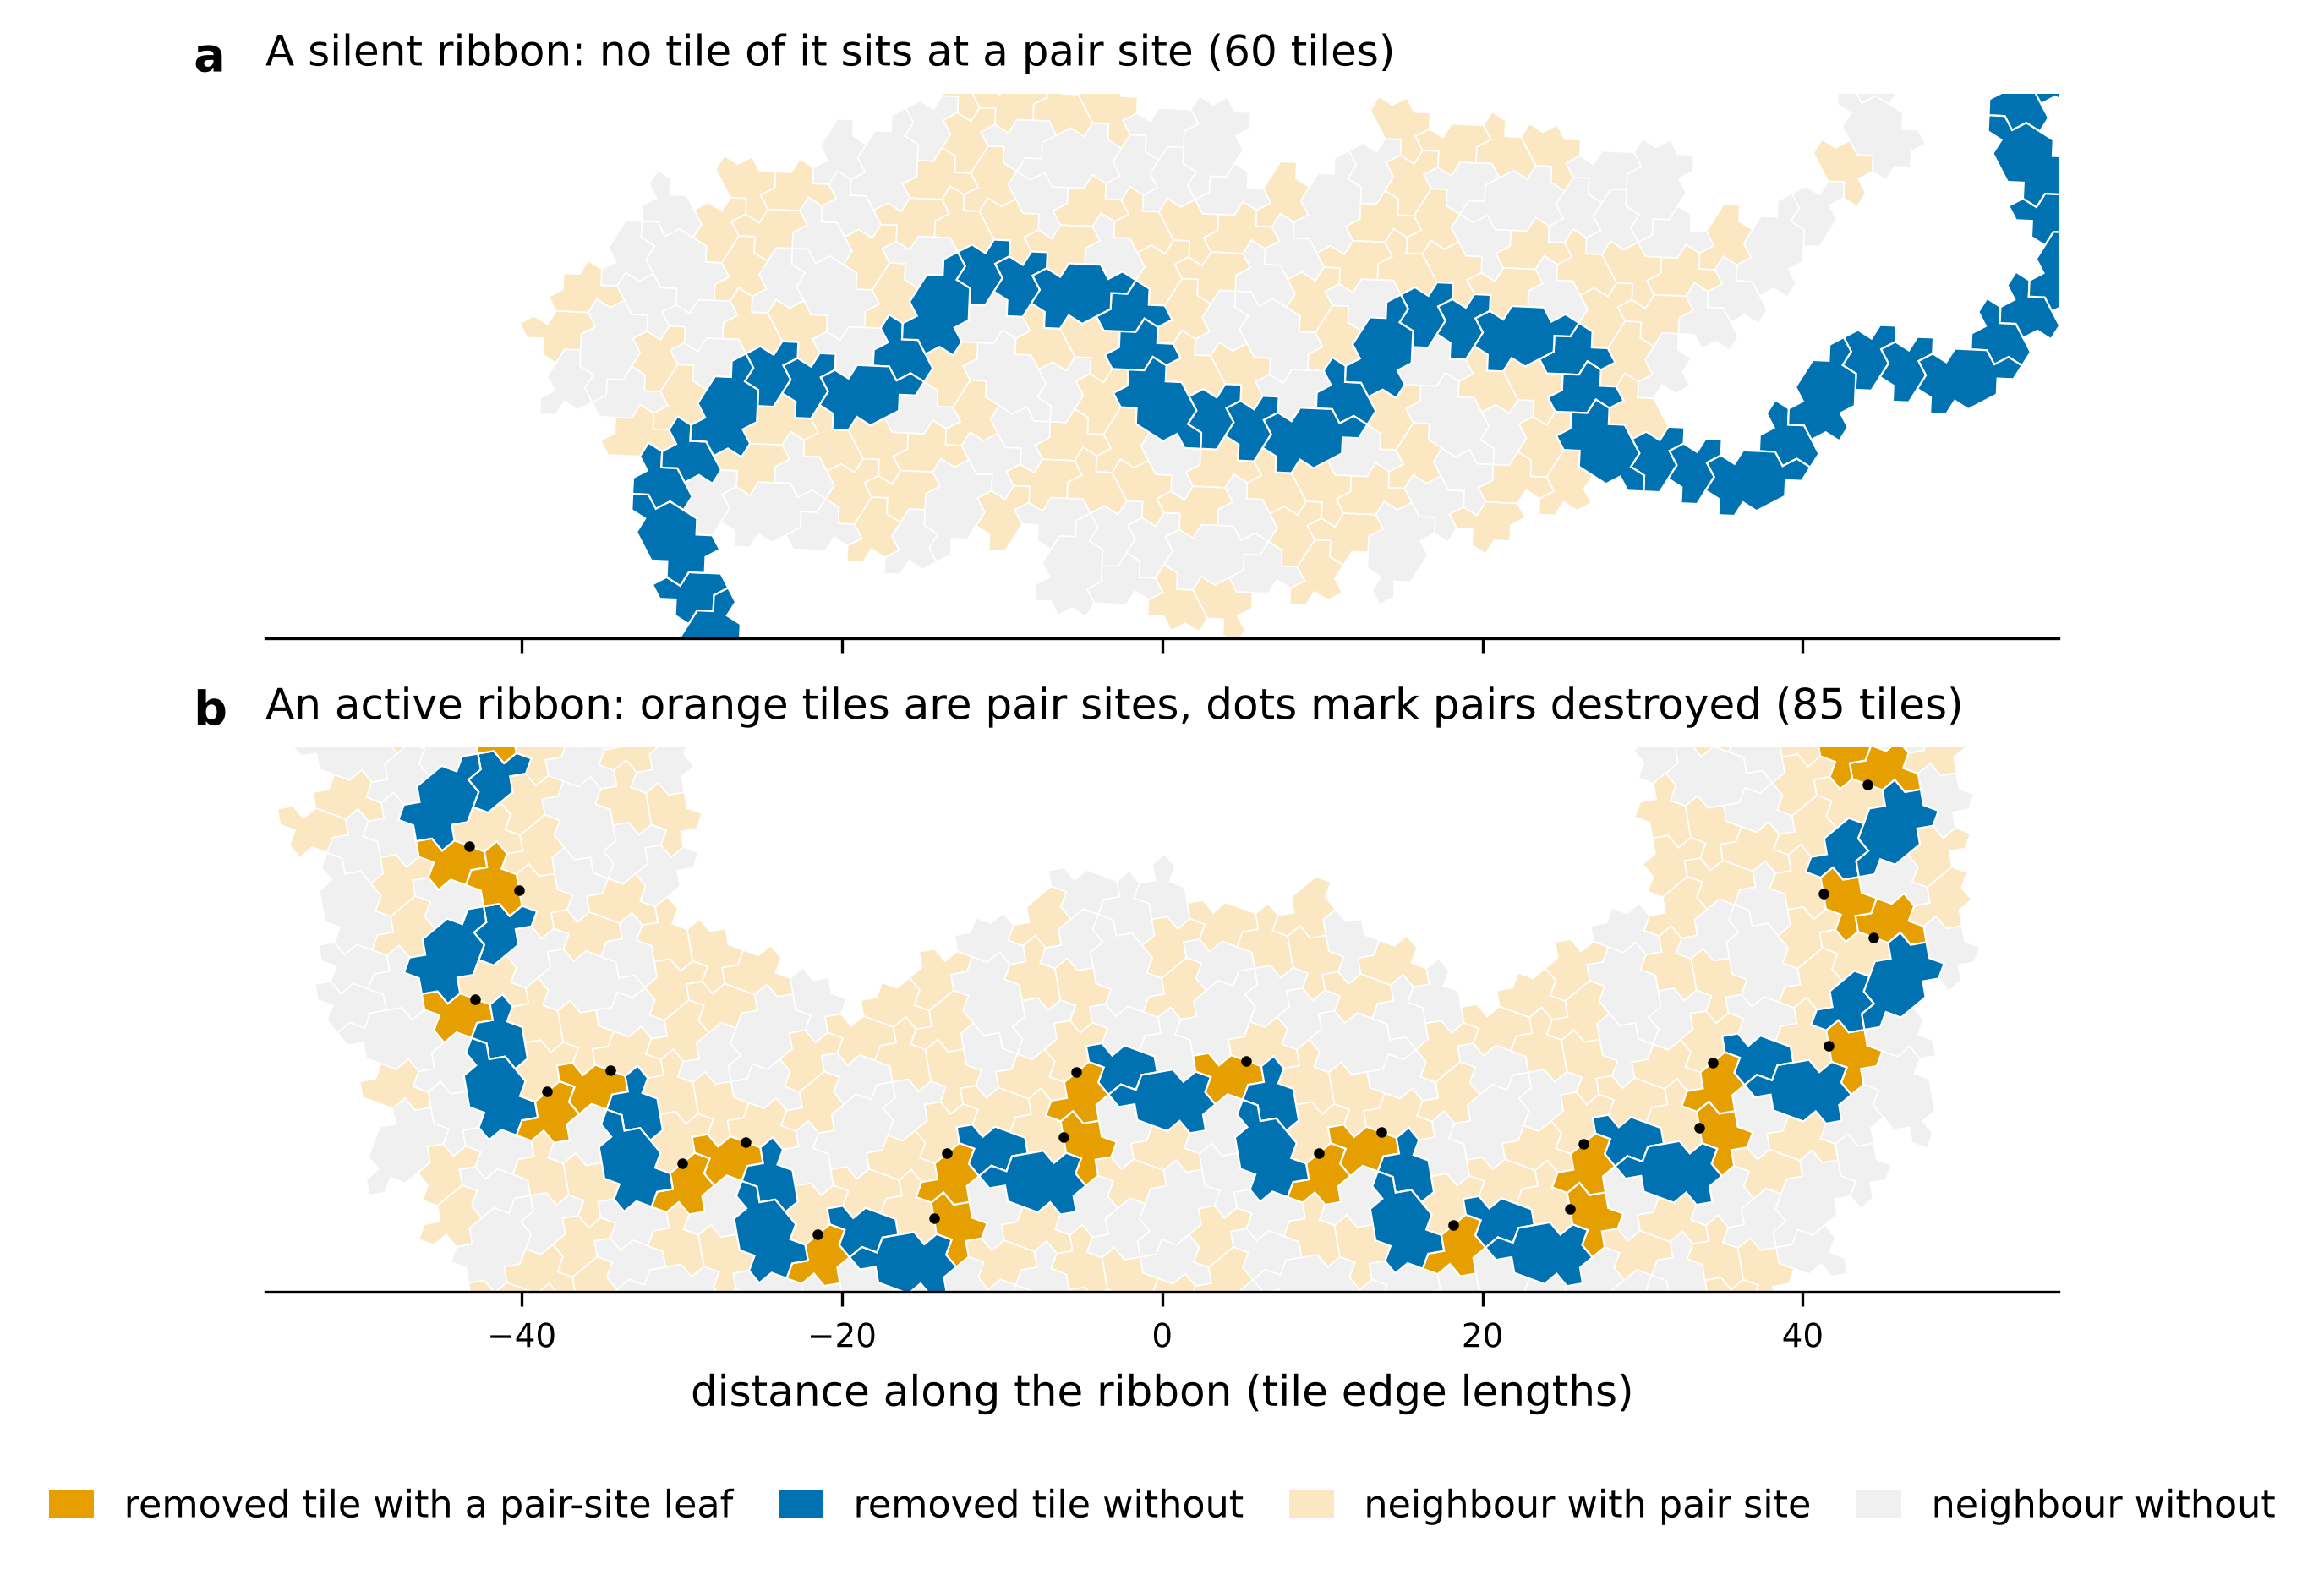
\includegraphics[width=\linewidth]{ribbon_1_silent_vs_active.png}
\caption{Two phason ribbons of the Spectre tiling, straightened along their axes. Blue: removed tiles with no pair site; orange: removed tiles at a pair site; pale tiles: neighbours with (orange) and without (grey) a pair site; dots: pairs destroyed. (a) A silent ribbon: it changes $60$ tiles and no pair. (b) An active ribbon: pairs are destroyed and created along it at $0.24$ per unit length each (Results~\ref{res:ribbon}--\ref{res:silent}).}\label{fig:ribbon}
\end{figure}

%------------------------------------------------------------------------------------------------------------------------------------
\section{On the sphere, flips are bits at the cone points}\label{sec:sphere}
At the Hat end of the flow the tile is a polykite \cite{smith2024hat} and can be placed on any surface that carries the kite grid. On the Goldberg sphere $GP(3,0)$ the $80$ hexagons give $480$ kites and the $12$ pentagons are left as holes; capping each hole gives a flat surface with $12$ cone points of deficit $60^\circ$, the intrinsic metric of the icosahedron \cite{thurston1998}.
\begin{result}[\exact]\label{res:register}
The sphere has exactly $4096=2^{12}$ hat tilings. The $480$ kites split into $12$ rings of $40$ kites, one around each cone point and the same in every tiling, and each ring is tiled by five hats in exactly two ways, independently of the others. Removing any connected set of up to seven hats from a symmetric tiling and re-tiling it finds no other flip. So the space of tilings is a register $\sigma\in\{0,1\}^{12}$, a flip is $X_p$ on one bit, every flip is a closed cluster of five tiles, and the two icosahedrally symmetric tilings are $\sigma=0$ and $\sigma=1$ (Figure~\ref{fig:rings}).
\end{result}
\begin{result}[\exact]\label{res:euler}
With hats and pentagons as faces, the counts are
\begin{equation}\label{eq:euler}
V(\sigma)=V_0-n_{11}(\sigma),\qquad E(\sigma)=E_0-n_{11}(\sigma),\qquad F=72,\qquad n_{11}(\sigma)=\sum_{\langle pq\rangle}\sigma_p\sigma_q ,
\end{equation}
with $V_0=140$, $E_0=210$ and the sum running over the $30$ edges of the icosahedron (each edge with both bits set carries one four-valent vertex). A flip at $p$ with $k$ of its five neighbours set changes $(V,E,F)$ by $(\mp k,\mp k,0)$; only $k=0$ is a Pachner-type $2\leftrightarrow2$ count.
\end{result}
\begin{figure}[t]\centering
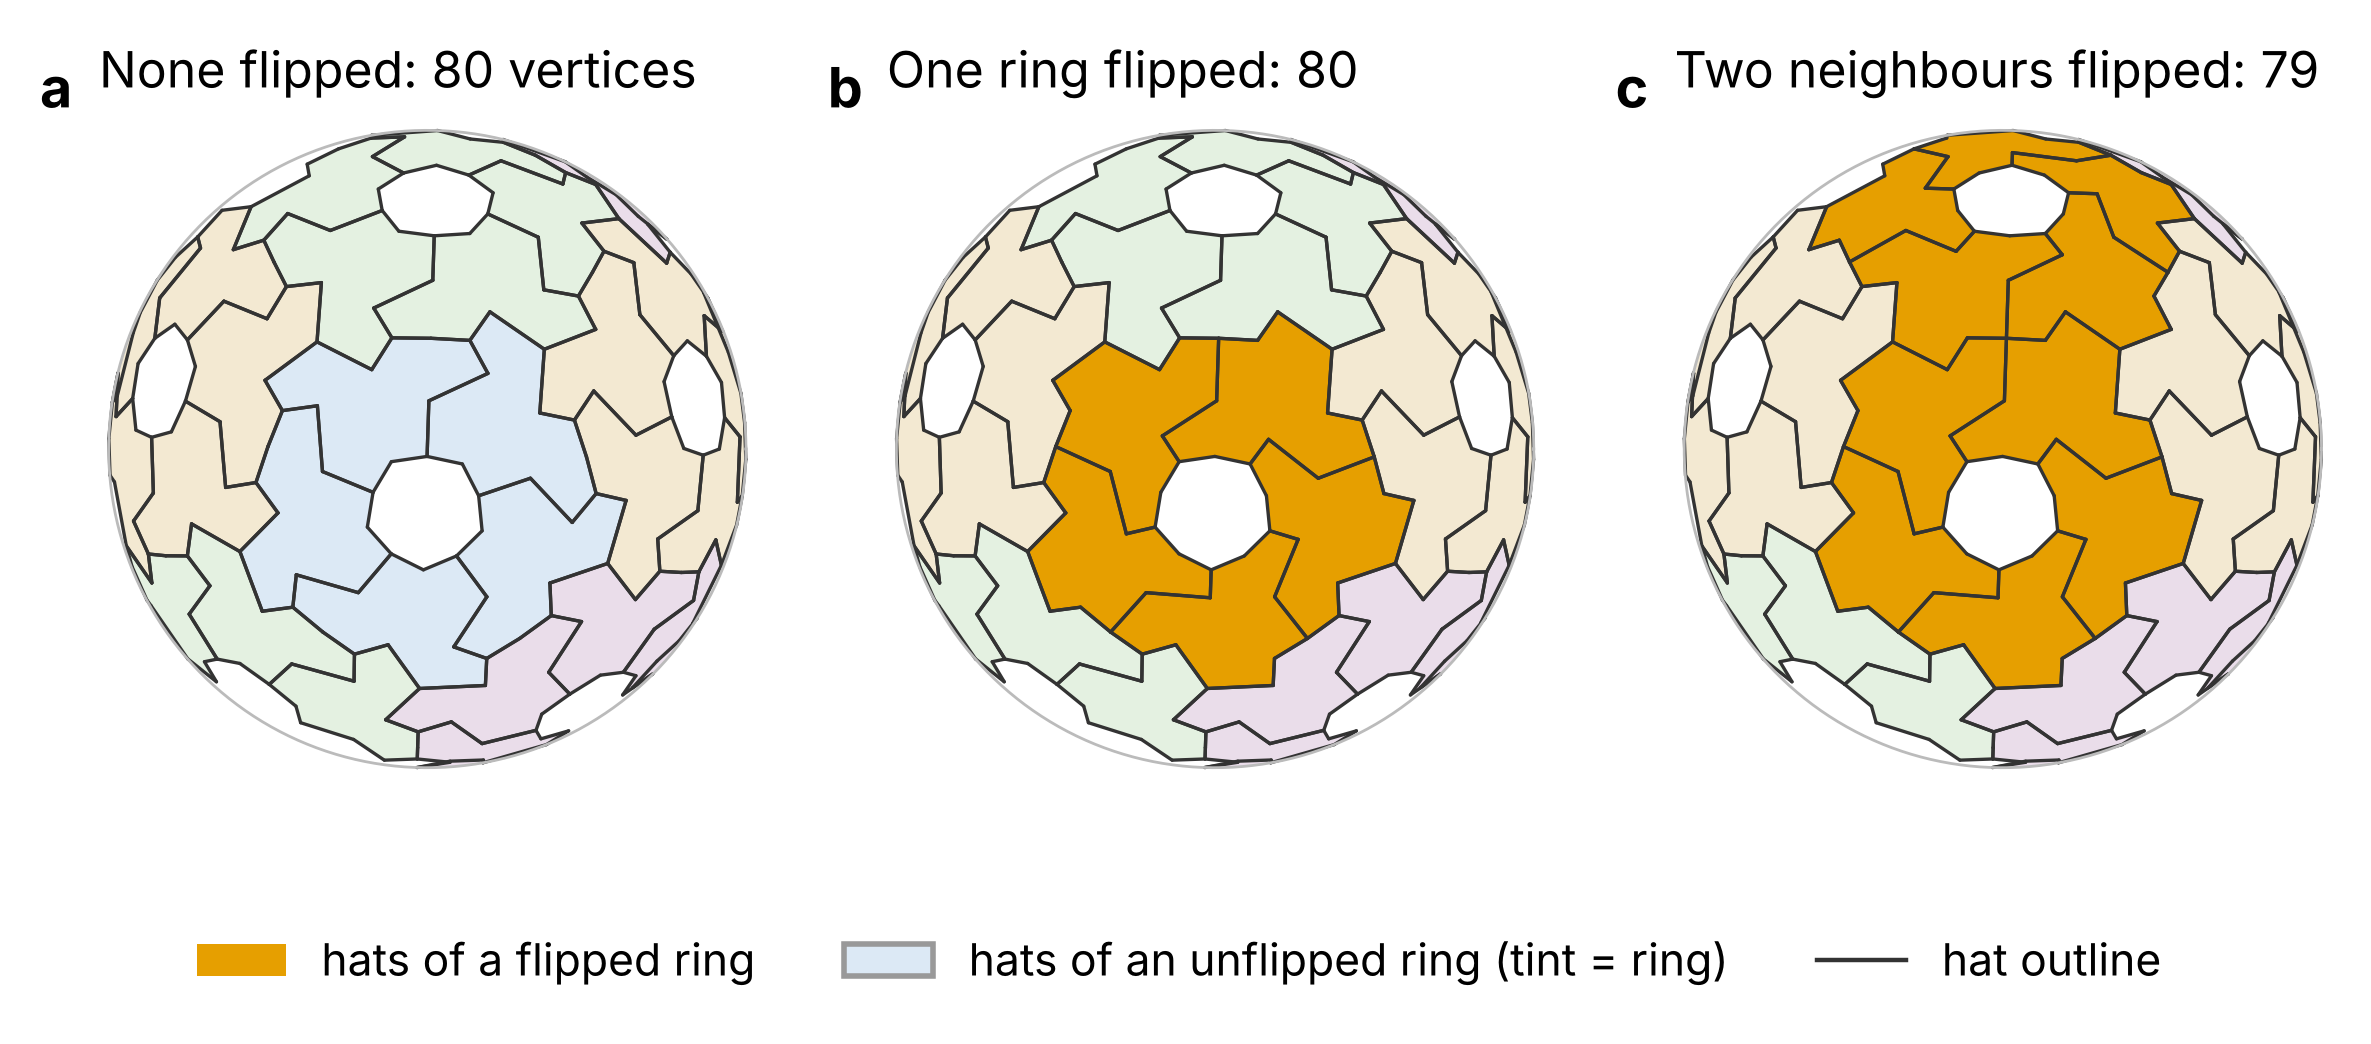
\includegraphics[width=\linewidth]{hat_time_1_rings.png}
\caption{The Hat Trick sphere seen from above one cone point (white: the $12$ pentagonal holes; tints: the rings of five hats). (a) $\sigma=0$. (b) One ring flipped: its outline is fixed and its five hats are cut the other way. (c) A neighbouring ring flipped as well: one vertex is lost, as Eq.~\eqref{eq:euler} says.}\label{fig:rings}
\end{figure}
The geometry is a $12$-qubit register and the matter sits on its edges: a pair exists on the icosahedron edge $e=pq$ iff $\sigma_p=\sigma_q=0$, so the all-$0$ tiling has $30$ pair qubits and the all-$1$ tiling none \cite{hexasphere}. Writing $n_e=(1-\sigma_p)(1-\sigma_q)$ for the presence of the slot on $e$, geometry and matter combine as
\begin{equation}\label{eq:joint}
H_{\mathrm{joint}}=\underbrace{-\Gamma\sum_pX_p+g\sum_p(1-\sigma_p)}_{\text{geometry: ring flips}}\;\underbrace{-\,J\sum_en_e\,\tau^x_e-\kappa\sum_{e<e'}n_en_{e'}W_{ee'}\,\tau^z_e\tau^z_{e'}}_{\text{matter: pair qubits where the geometry allows}} ,
\end{equation}
where a slot keeps its state while it is switched off.
\begin{result}[\exact; \defn\ for $\Gamma$, $g$]\label{res:joint}
$X_p$ permutes the basis states of geometry and slots, so a flip is unitary and its own inverse on a fixed finite space, with no boundary term and no conserved pair number. At $\kappa=0$ and with all slots in $|+\rangle$ the geometry alone is $-\Gamma\sum X_p+g\sum(1-\sigma_p)-J\sum_{\langle pq\rangle}(1-\sigma_p)(1-\sigma_q)$, at $g=5J/2$ the transverse-field Ising model on the icosahedron, whose two ordered states are the two symmetric tilings. The number of pair qubits and of vertices are then observables with a quantum spread (\numeric: at $g=0$, $\Gamma=3$, $J=1$ the mean pair number is $17.8$ of $30$).
\end{result}
Two limits of this closed substrate matter. Its curvature is a fixed background: the cone points belong to the kite grid, no re-tiling moves them, and no other Goldberg sphere with odd $T\le39$ carries a hat tiling (\exact). On closed folds of Spectre patches \cite{ballgen} the cone points do move under local changes of the patch ($22\%$ of local swaps must change the multiset of deficits), and an exact search for second tilings finds flips only in clusters that contain a cone point ($151$ of $1079$ clusters of two to four tiles, against none of $1243$ without one; \numeric, the search misses some tilings, so these are lower bounds). On both closed surfaces the flips that close sit at cone points.

%------------------------------------------------------------------------------------------------------------------------------------
\section{Gauge invariance and quantisation}\label{sec:quant}
\begin{result}[\exact; \defn\ for the reading of a bit as a spin]\label{res:punctures}
The $60$ rotations of the icosahedron permute the bits and flip none. Read each bit as a spin-$\tfrac12$ at its cone point, $\sigma_p=\tfrac12(1-Z_p)$. The gauge-invariant space of a sphere with $12$ spin-$\tfrac12$ punctures, the $132$ singlets of $(\mathbb{C}^2)^{\otimes12}$, then lies in the span of the tilings with six bits set, and with $\Pi$ the projector onto it
\begin{equation}\label{eq:chain}
\Pi\,n_{11}\,\Pi=\sum_{\langle pq\rangle}\Bigl(\tfrac14+\tfrac13\,\vec S_p\cdot\vec S_q\Bigr)=\tfrac{15}2+\tfrac13\sum_{\langle pq\rangle}\vec S_p\cdot\vec S_q ,
\end{equation}
because $\Pi Z_p\Pi=0$ and $\Pi Z_pZ_q\Pi=\tfrac43\,\Pi\,\vec S_p\cdot\vec S_q\,\Pi$ by rotation invariance (checked to $10^{-13}$). The vertex count of Eq.~\eqref{eq:euler} becomes the antiferromagnetic Heisenberg model on the icosahedron; its lowest level, $\sum\vec S_p\cdot\vec S_q=-6.1879$, is unique.
\end{result}
A quantum Hamiltonian thus appears without a transverse field put in by hand: a geometric count plus gauge invariance. A single bit is not gauge invariant, as a single pair qubit is not; only the $132$ combinations are.

The singlets are the non-crossing pairings of $12$ points and $\vec S_p\cdot\vec S_q=\tfrac14-\tfrac12e_{pq}$, with $e_{pq}$ twice the singlet projector: a Temperley--Lieb algebra \cite{temperleylieb1971} at loop value $2$. Its Kauffman-bracket deformation \cite{kauffman1987} is the skein quantisation of the Poisson algebra of loops \cite{turaev1991,bullock2000}, which Asselmeyer-Maluga and Kr\'ol use to argue that wild embeddings are quantum states \cite{asselmeyer2013,asselmeyer2019}. We apply the same deformation to our twelve punctures, with no wild embedding:
\begin{equation}\label{eq:levels}
\begin{gathered}
H_k=\sum_{\langle pq\rangle}\Bigl(\tfrac14-\frac{e_{pq}}{d_k}\Bigr),\qquad d_k=-A^2-A^{-2}=2\cos\frac{\pi}{k+2},\qquad A=i\,e^{i\pi/(2k+4)},\\
e_{pq}=\beta_{pq}^{-1}\,e_{i,i+1}\,\beta_{pq},\qquad \lim_{k\to\infty}H_k=\sum_{\langle pq\rangle}\vec S_p\cdot\vec S_q .
\end{gathered}
\end{equation}
Here the punctures are ordered along a Hamiltonian cycle of the icosahedron, and an edge that is not on the cycle is brought next to its partner by a braid $\beta_{pq}$ that passes over the strands on one side of the cycle and under those on the other (\defn).
\begin{result}[\exact]\label{res:levels}
The form on the pairing basis is positive and $H_k$ is self-adjoint for it at every level tested; the spectrum is the same for two different Hamiltonian cycles. The physical space at level $k$ has dimension $1$, $32$, $89$, $122$, $131$ for $k=1,\dots,5$ and $132$ from $k=6$ on, the Verlinde count \cite{verlinde1988} of $12$ spin-$\tfrac12$ insertions. The lowest level of $H_k$ is unique and moves smoothly to the classical value: $-14.208$ ($k=2$), $-8.525$ ($6$), $-6.668$ ($20$), $-6.196$ ($200$), $-6.1879$ ($k=\infty$) (Figure~\ref{fig:levels}).
\end{result}
\begin{result}[\exact]\label{res:majorana}
At level $2$ the operators $\Gamma_{pq}=2e_{pq}/d_2-1$ square to $1$, anticommute when two edges share a cone point and commute otherwise. Hence $\Gamma_{pq}=i\,s_{pq}\gamma_p\gamma_q$ with one Majorana operator $\gamma_p$ per cone point, signs $s_{pq}=\pm1$, and
\begin{equation}\label{eq:majorana}
\begin{gathered}
H_2=-\frac{15}2-\frac i2\sum_{\langle pq\rangle}s_{pq}\,\gamma_p\gamma_q,\qquad \Gamma_{pq}\Gamma_{qr}\Gamma_{rp}=\Phi\ \text{on all } 20 \text{ faces},\\
a^2=-5\ \ (a_{pq}=s_{pq}=-a_{qp}),\qquad E_m=-\frac{15}2+\frac{\sqrt5}2\,(6-2m),\quad m=0,2,4,6.
\end{gathered}
\end{equation}
The flux $\Phi=\pm i$ is the same on every face, all six fermion modes have energy $\sqrt5$, and the levels $-14.208$, $-9.736$, $-5.264$, $-0.792$ have $1$, $15$, $15$, $1$ states. The $32$ states are those of $12$ Ising anyons \cite{kitaev2006}: five qubits on pairs of neighbouring cone points. A single ring flip has no level-$2$ form, since one $\gamma_p$ changes the fermion parity.
\end{result}
\begin{figure}[t]\centering
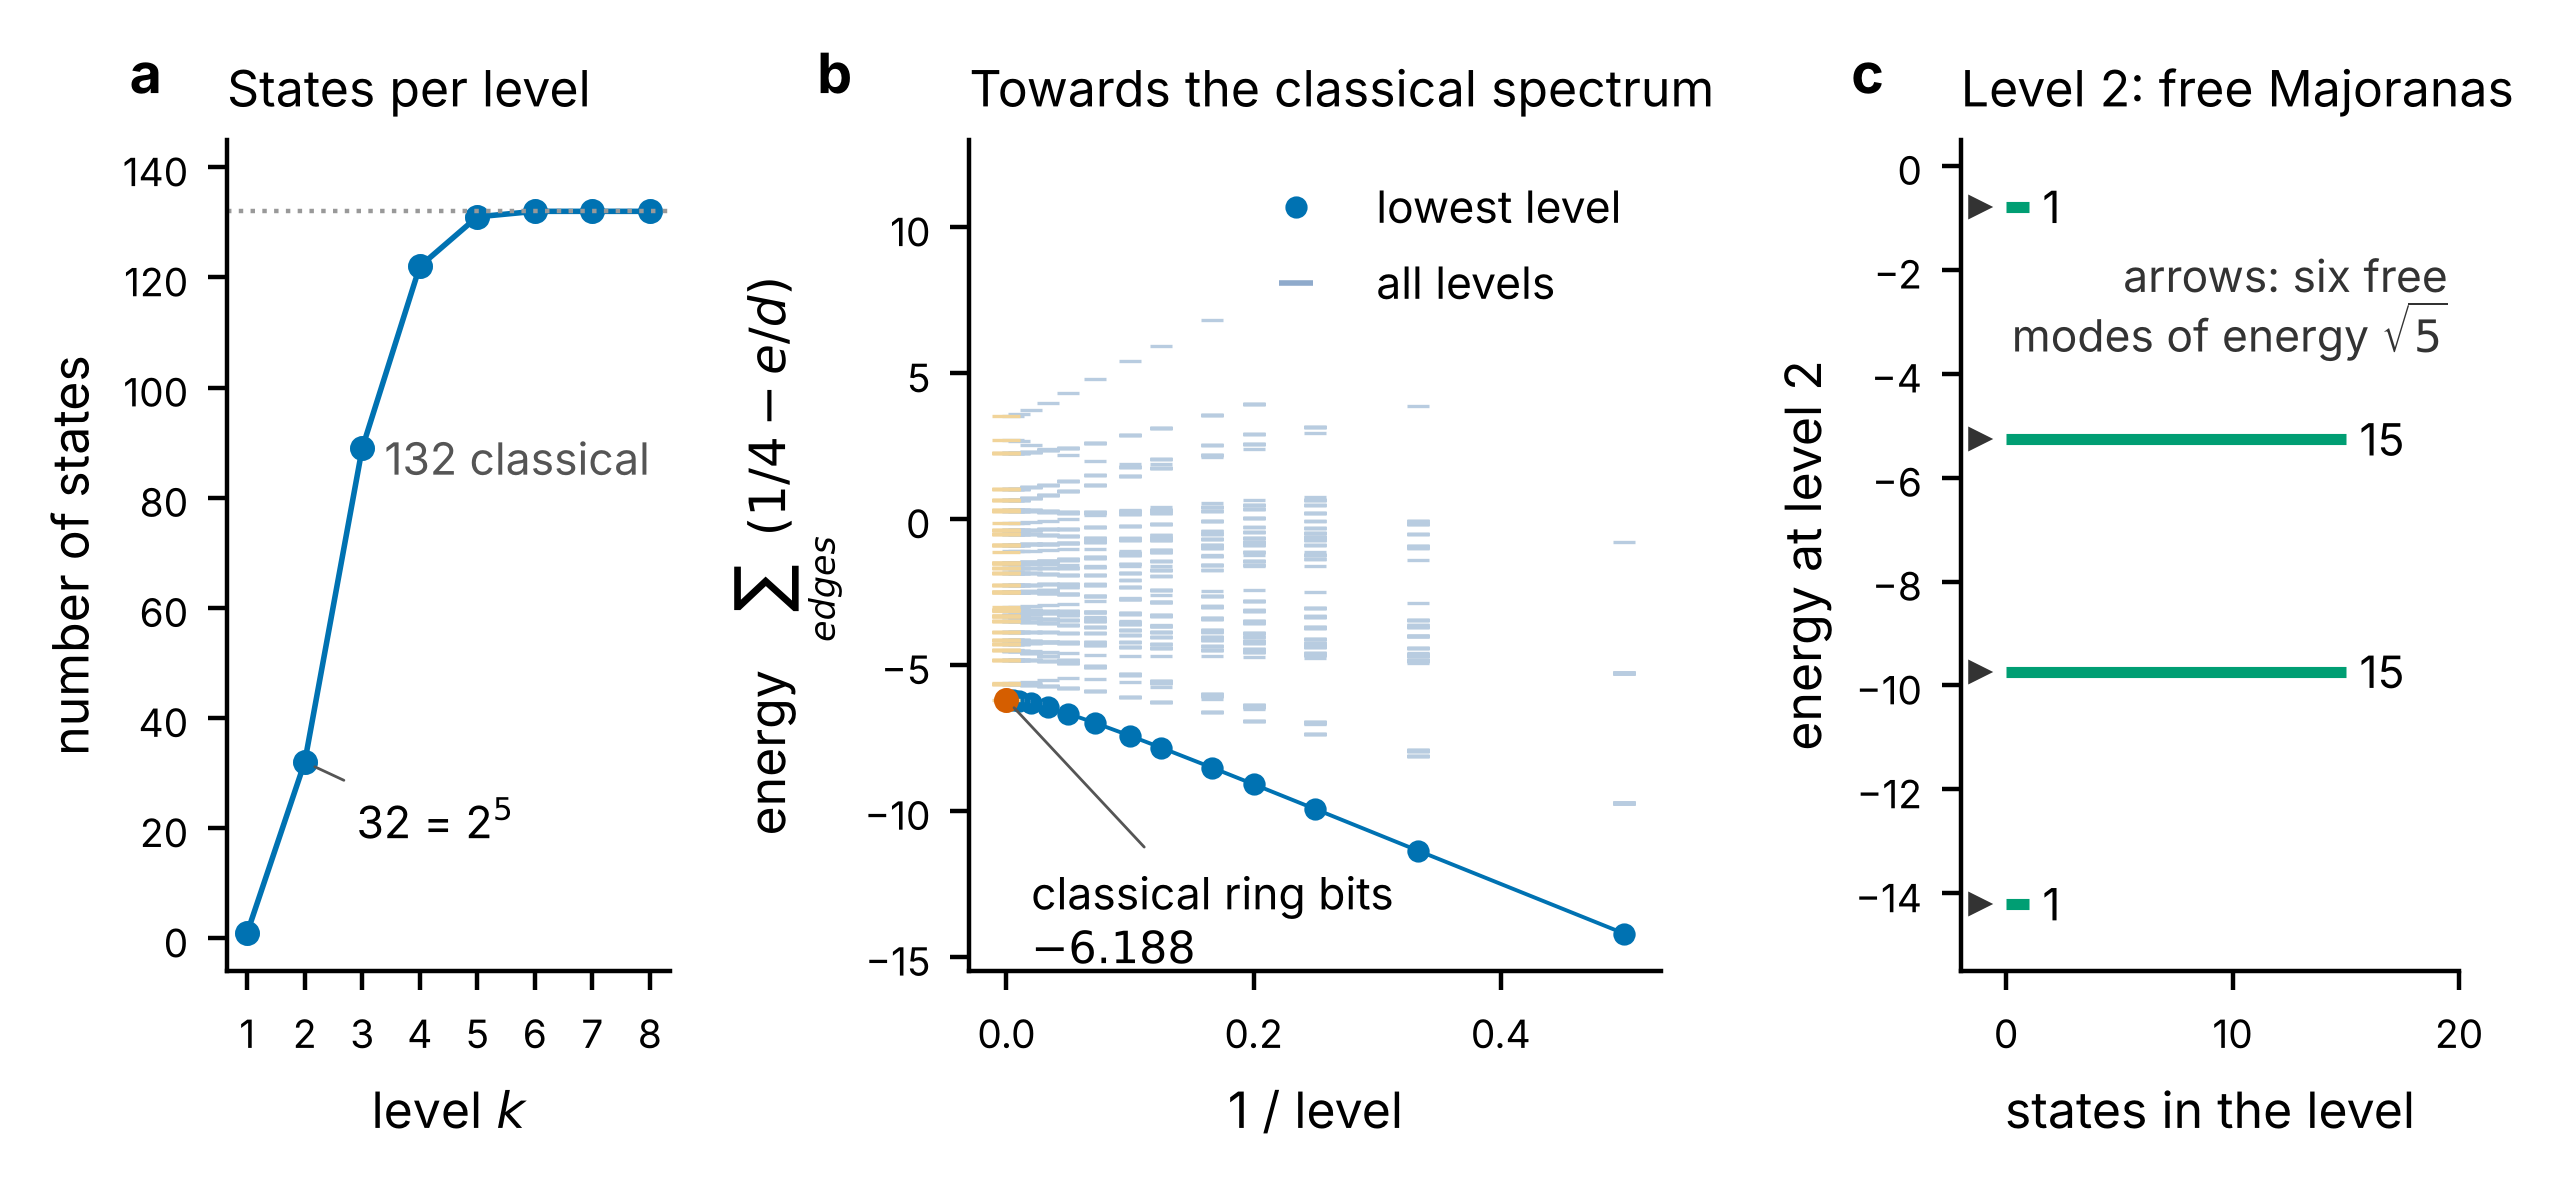
\includegraphics[width=\linewidth]{hat_time_2_levels.png}
\caption{Quantisation levels of the twelve punctures. (a) Dimension of the state space at level $k$. (b) All levels of $H_k$ against $1/k$ (dots: lowest level), tending to the Heisenberg spectrum of Eq.~\eqref{eq:chain} (orange). (c) Level $2$: four levels with $1$, $15$, $15$, $1$ states, as predicted by six free Majorana modes of energy $\sqrt5$ (arrows).}\label{fig:levels}
\end{figure}

%------------------------------------------------------------------------------------------------------------------------------------
\section{Two kinds of handedness}\label{sec:hands}
\begin{result}[\exact]\label{res:flux}
The sign of $\Phi$ is fixed by the orientation used to braid: with the braid passing over the strands on the left of the cycle, seen from outside, $\Phi=-i$ for either cycle and either direction, and $\Phi$ changes sign when over and under are exchanged and when $A\mapsto A^{-1}$. Nothing else enters.
\end{result}
The hat itself has a hand: all $4096$ tilings use one hand of the tile. The question is whether that hand fixes $\Phi$.
\begin{result}[\numeric]\label{res:chi4}
A reflection $R$ of the icosahedron permutes the bits. For $1320$ of the $4096$ bit strings the mirrored string is not a rotation of the original, and for all $1320$ the two tilings differ as cell complexes: the hat's hand is visible in the bits. Counting tiles by their surroundings, the difference first appears at the third neighbours ($93$ of $124$ counts acquire a mirror-odd part), and as a polynomial in the bits every mirror-odd part starts at order four. The simplest such term is
\begin{equation}\label{eq:chi4}
\chi_4(\sigma)=\sum_{a\text{-}b\text{-}c\text{-}d}h_{abcd}\,\sigma_a\sigma_b\sigma_c\sigma_d,\qquad h_{abcd}=\begin{cases}+1&\text{the path turns left at } b\\-1&\text{the path turns right at } b\end{cases}
\end{equation}
over the $60$ paths of three edges from a vertex of the icosahedron to its antipode ($30$ of each hand; Figure~\ref{fig:chirality}). It is invariant under the $60$ rotations, odd under $R$, takes the values $-1,0,+1$ on $480$, $3136$, $480$ strings, and is the whole order-four mirror-odd part of $15$ of the counts. The vertex count, and with it every Hamiltonian above, is even under $R$.
\end{result}
\begin{figure}[t]\centering
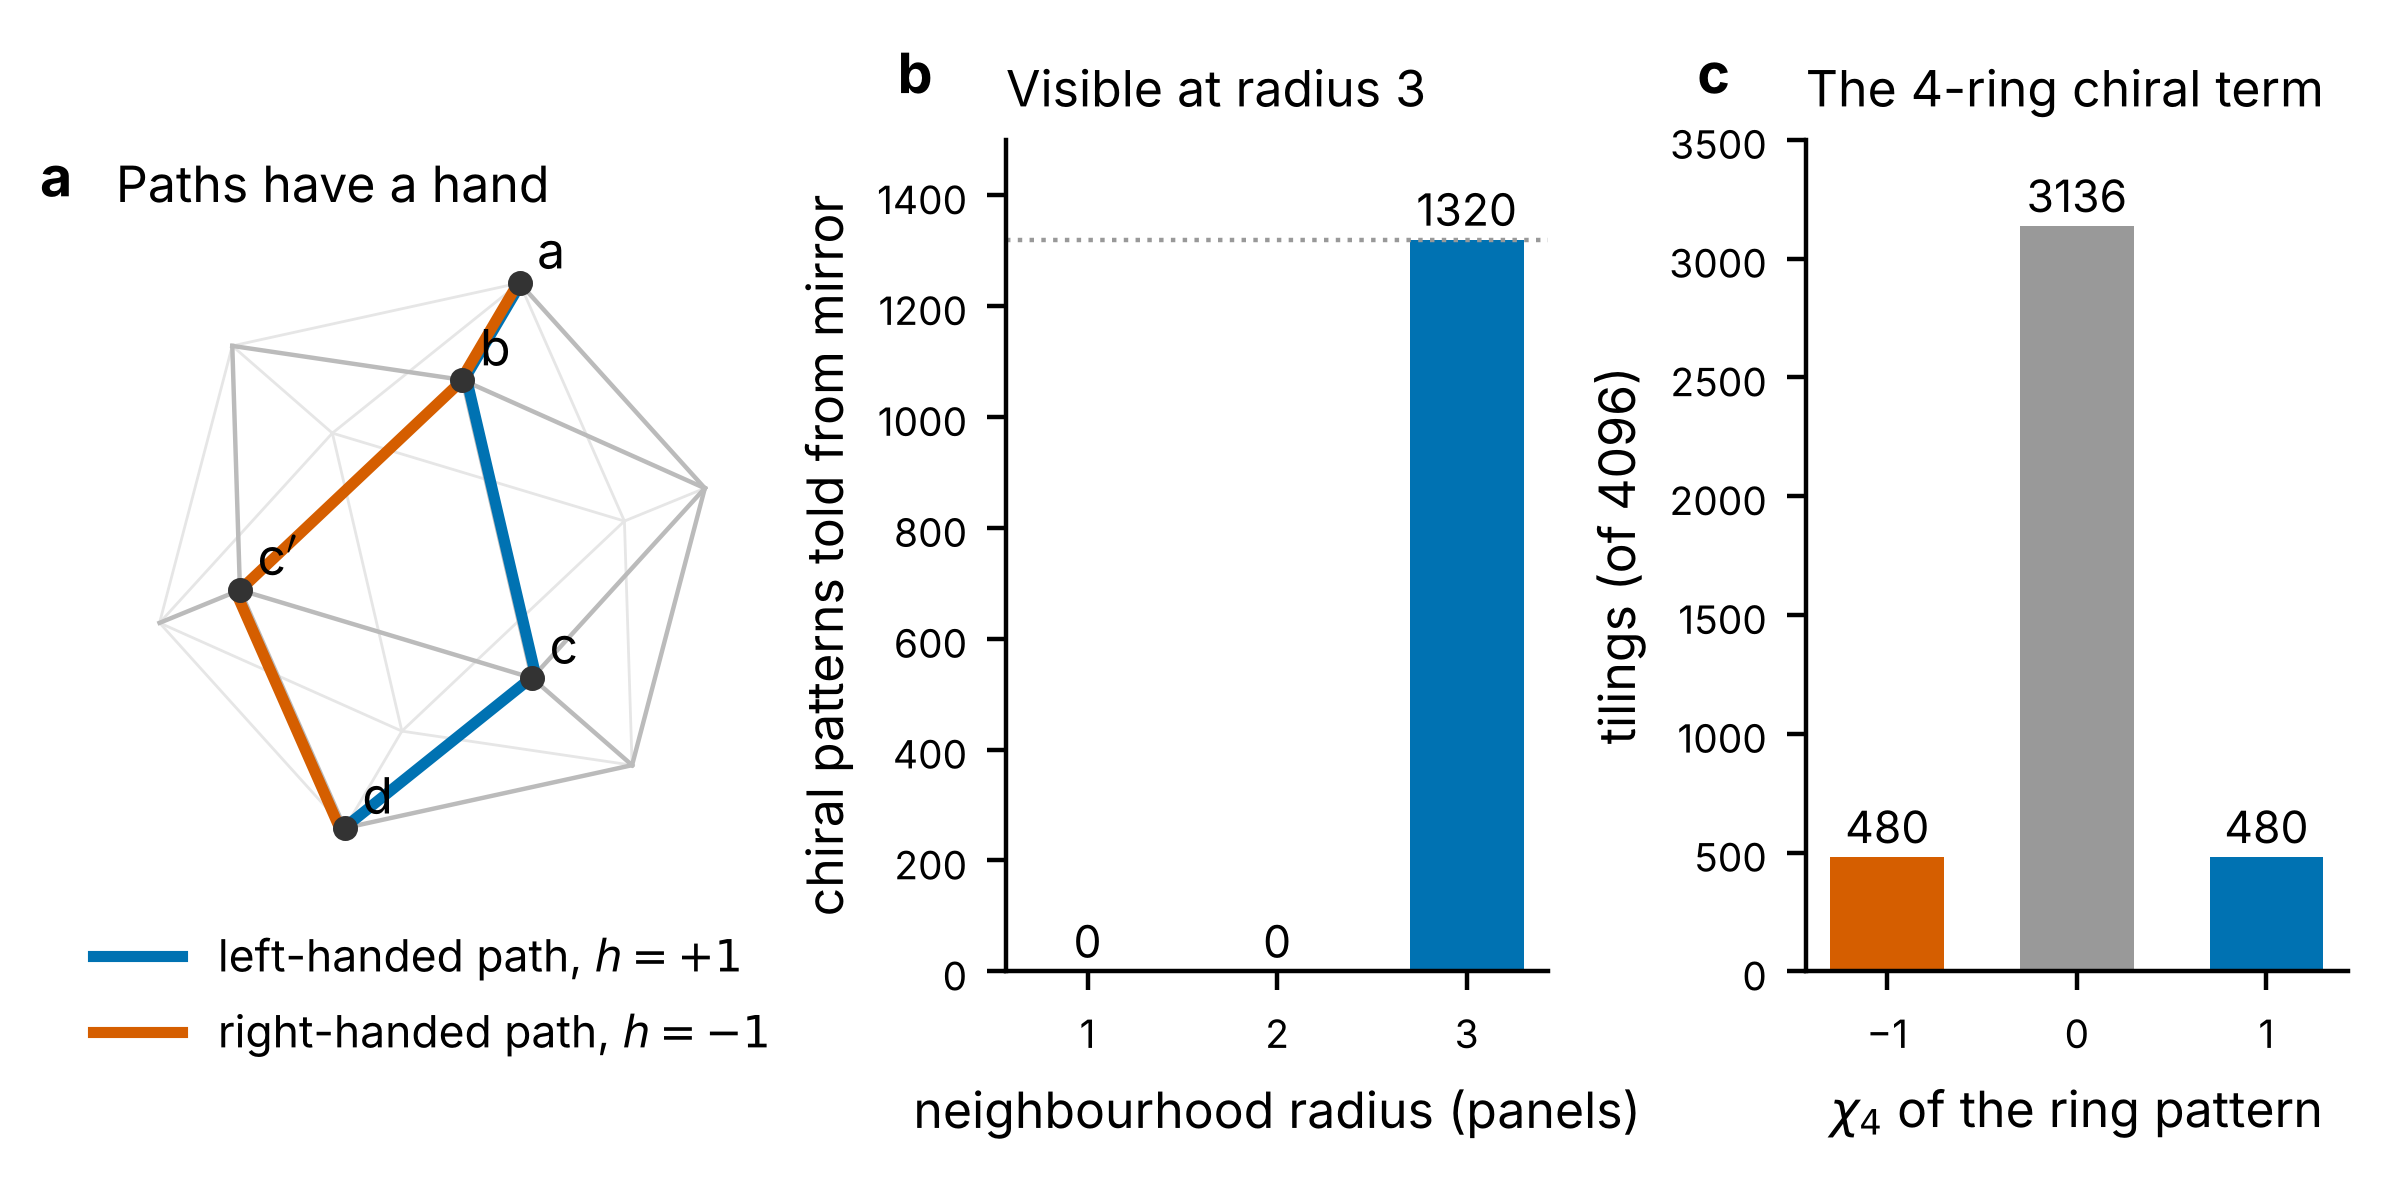
\includegraphics[width=\linewidth]{hat_time_3_chirality.png}
\caption{The hat's hand in the bits. (a) Two paths from a vertex $a$ to its antipode $d$ through the same $b$: one turns left at $b$ ($h=+1$), one right ($h=-1$). (b) Mirror pairs of bit strings whose tilings can be told apart, by counting tiles by their surroundings out to $1$, $2$, $3$ neighbours. (c) Values of $\chi_4$ over all $4096$ tilings.}\label{fig:chirality}
\end{figure}
Let $K$ be complex conjugation in the tiling basis. Every function of the tiling, $\chi_4$ included, is a real diagonal operator in that basis, so it is even under $K$. The flux is not: $A\mapsto A^{-1}=\bar A$ is complex conjugation of the level-$k$ operators, and it reverses $\Phi$ (Result~\ref{res:flux}). Under the two reflections
\begin{equation}\label{eq:hands}
R:\ (\chi_4,\Phi)\mapsto(-\chi_4,-\Phi),\qquad K:\ (\chi_4,\Phi)\mapsto(\chi_4,-\Phi),\qquad RK:\ (\chi_4,\Phi)\mapsto(-\chi_4,\Phi).
\end{equation}
A term in the energy linear in both, $c\,\chi_4\,\Phi$, is odd under $K$, so it vanishes in any description that is symmetric under $K$. The hat breaks mirror symmetry; the flux needs, in addition, time reversal broken, and that is what choosing the sign of the level does. If $K$ is read as time reversal, the tiling supplies a spatial hand and not an arrow. This is a symmetry argument: $\chi_4$ has not been built as an operator on the $132$ singlets or on the level-$2$ states.

%------------------------------------------------------------------------------------------------------------------------------------
\section{Discussion}\label{sec:discussion}
The model has a substrate (a model set with an exact window), matter (dipolar pair qubits whose couplings come from the tile areas), a geometry whose moves are exact and unitary on a closed surface, and a quantisation of that geometry whose classical limit is the vertex count. Three features are, to our knowledge, not found in other discrete models: the flips of the plane are open ribbons whose action on the matter is decided by the window position; on the sphere the space of geometries is exactly one bit per unit of curvature; and the tiling's chirality and the chirality of the quantised theory are distinct, with only the second tied to time reversal.

The standard diagnostics give limited answers, and we only summarise them. The relative entropy of a region of pair qubits follows its volume, not its boundary; no area observable of the model is proportional to it; and the local first law $K_A\approx\beta H_A$ holds only for a hot reference state, whatever the sign of $\beta$ \cite{doraumuch}. The two-qubit Hopf map $S^7\to S^4$ applies to a pair exactly when the pair is pure. Planar flips have no arrow of time, because the flip relation is symmetric; the sphere's dynamics has none either, since $H_{\mathrm{joint}}$ is real.

The connection to wild embeddings is through the algebra only. Asselmeyer-Maluga and Kr\'ol identify the quantisation of a tame embedding with a wild one by way of the Temperley--Lieb tower and its type $\mathrm{II}_1$ limit \cite{asselmeyer2013,jones1983}; the step from the horned sphere to marked points is by analogy there. Our twelve punctures are tame, a Cantor set in a surface is always tame, and the $\mathrm{II}_1$ limit would need cone points at more and more scales, which the hat sphere does not have.

%------------------------------------------------------------------------------------------------------------------------------------
\section{Conclusion}\label{sec:conclusion}
The monotile tilings give a quantum-geometry model whose main pieces, the moves, the register and the couplings, come from the tiling itself. In the plane the moves of the tiling are open ribbons: they never close into local clusters, yet they act on the pair qubits locally and at a fixed rate, and the fractal window decides where. On a closed surface the moves close, and the counting becomes exact: the hat sphere is a register of one bit per cone point, each flip is a closed ring with an exact Euler change, and the degrees of freedom sit where the curvature is, although the curvature itself does not move. Gauge invariance turns that register into the twelve-puncture space and the vertex count into the Heisenberg model on the icosahedron, and the skein quantisation continues it to a family of levels whose level-$2$ member is a free Majorana model with a uniform flux.

The model separates two things that are easy to conflate. The tile's chirality is a property of space: it is visible in the tilings through a four-bit term on helical paths and leaves every Hamiltonian above unchanged. The chirality of the quantised theory, the sign of the flux, is tied to complex conjugation and so to time reversal, and the tiling does not choose it. What the model lacks for gravity is equally clear: the curvature on the sphere is fixed, the scales $\Gamma$, $g$, $\kappa$ and the level $k$ are put in by hand, no area law or Newtonian limit appears, and nothing distinguishes a direction of time. The next steps are therefore concrete:
\begin{enumerate}[leftmargin=1.6em,itemsep=1pt]
\item Are the planar ribbons infinite? They reach radius $100$ in one phase; a proof would need the geometry of the window.
\item $\chi_4$ as an operator on the gauge-invariant and level-$2$ spaces, and whether the one-handed Spectre gives a term of the same kind on its closed folds.
\item A converged ground state of Eq.~\eqref{eq:joint} at $\kappa\neq0$, and values of $\Gamma$, $g$ and the level $k$ from the geometry rather than by choice.
\item A closed substrate with both movable cone points and many pair qubits: the hat sphere has the second, the Spectre folds the first.
\end{enumerate}
\bibliographystyle{plain}
\bibliography{quantgrav}

\end{document}
